\documentclass{article}

\usepackage{graphicx}
\usepackage{tikz}
\usepackage{tikzsymbols}
\usetikzlibrary{calc,patterns,shapes.geometric}
\pagestyle{empty}
\usepackage[margin=0pt]{geometry}
\geometry{papersize={14in,12in}}

\def\centerarc[#1](#2)(#3:#4:#5){\draw[#1] ($(#2)+({#5*cos(#3)},{#5*sin(#3)})$) arc (#3:#4:#5);}

\begin{document}
	\begin{figure}
		\centering
		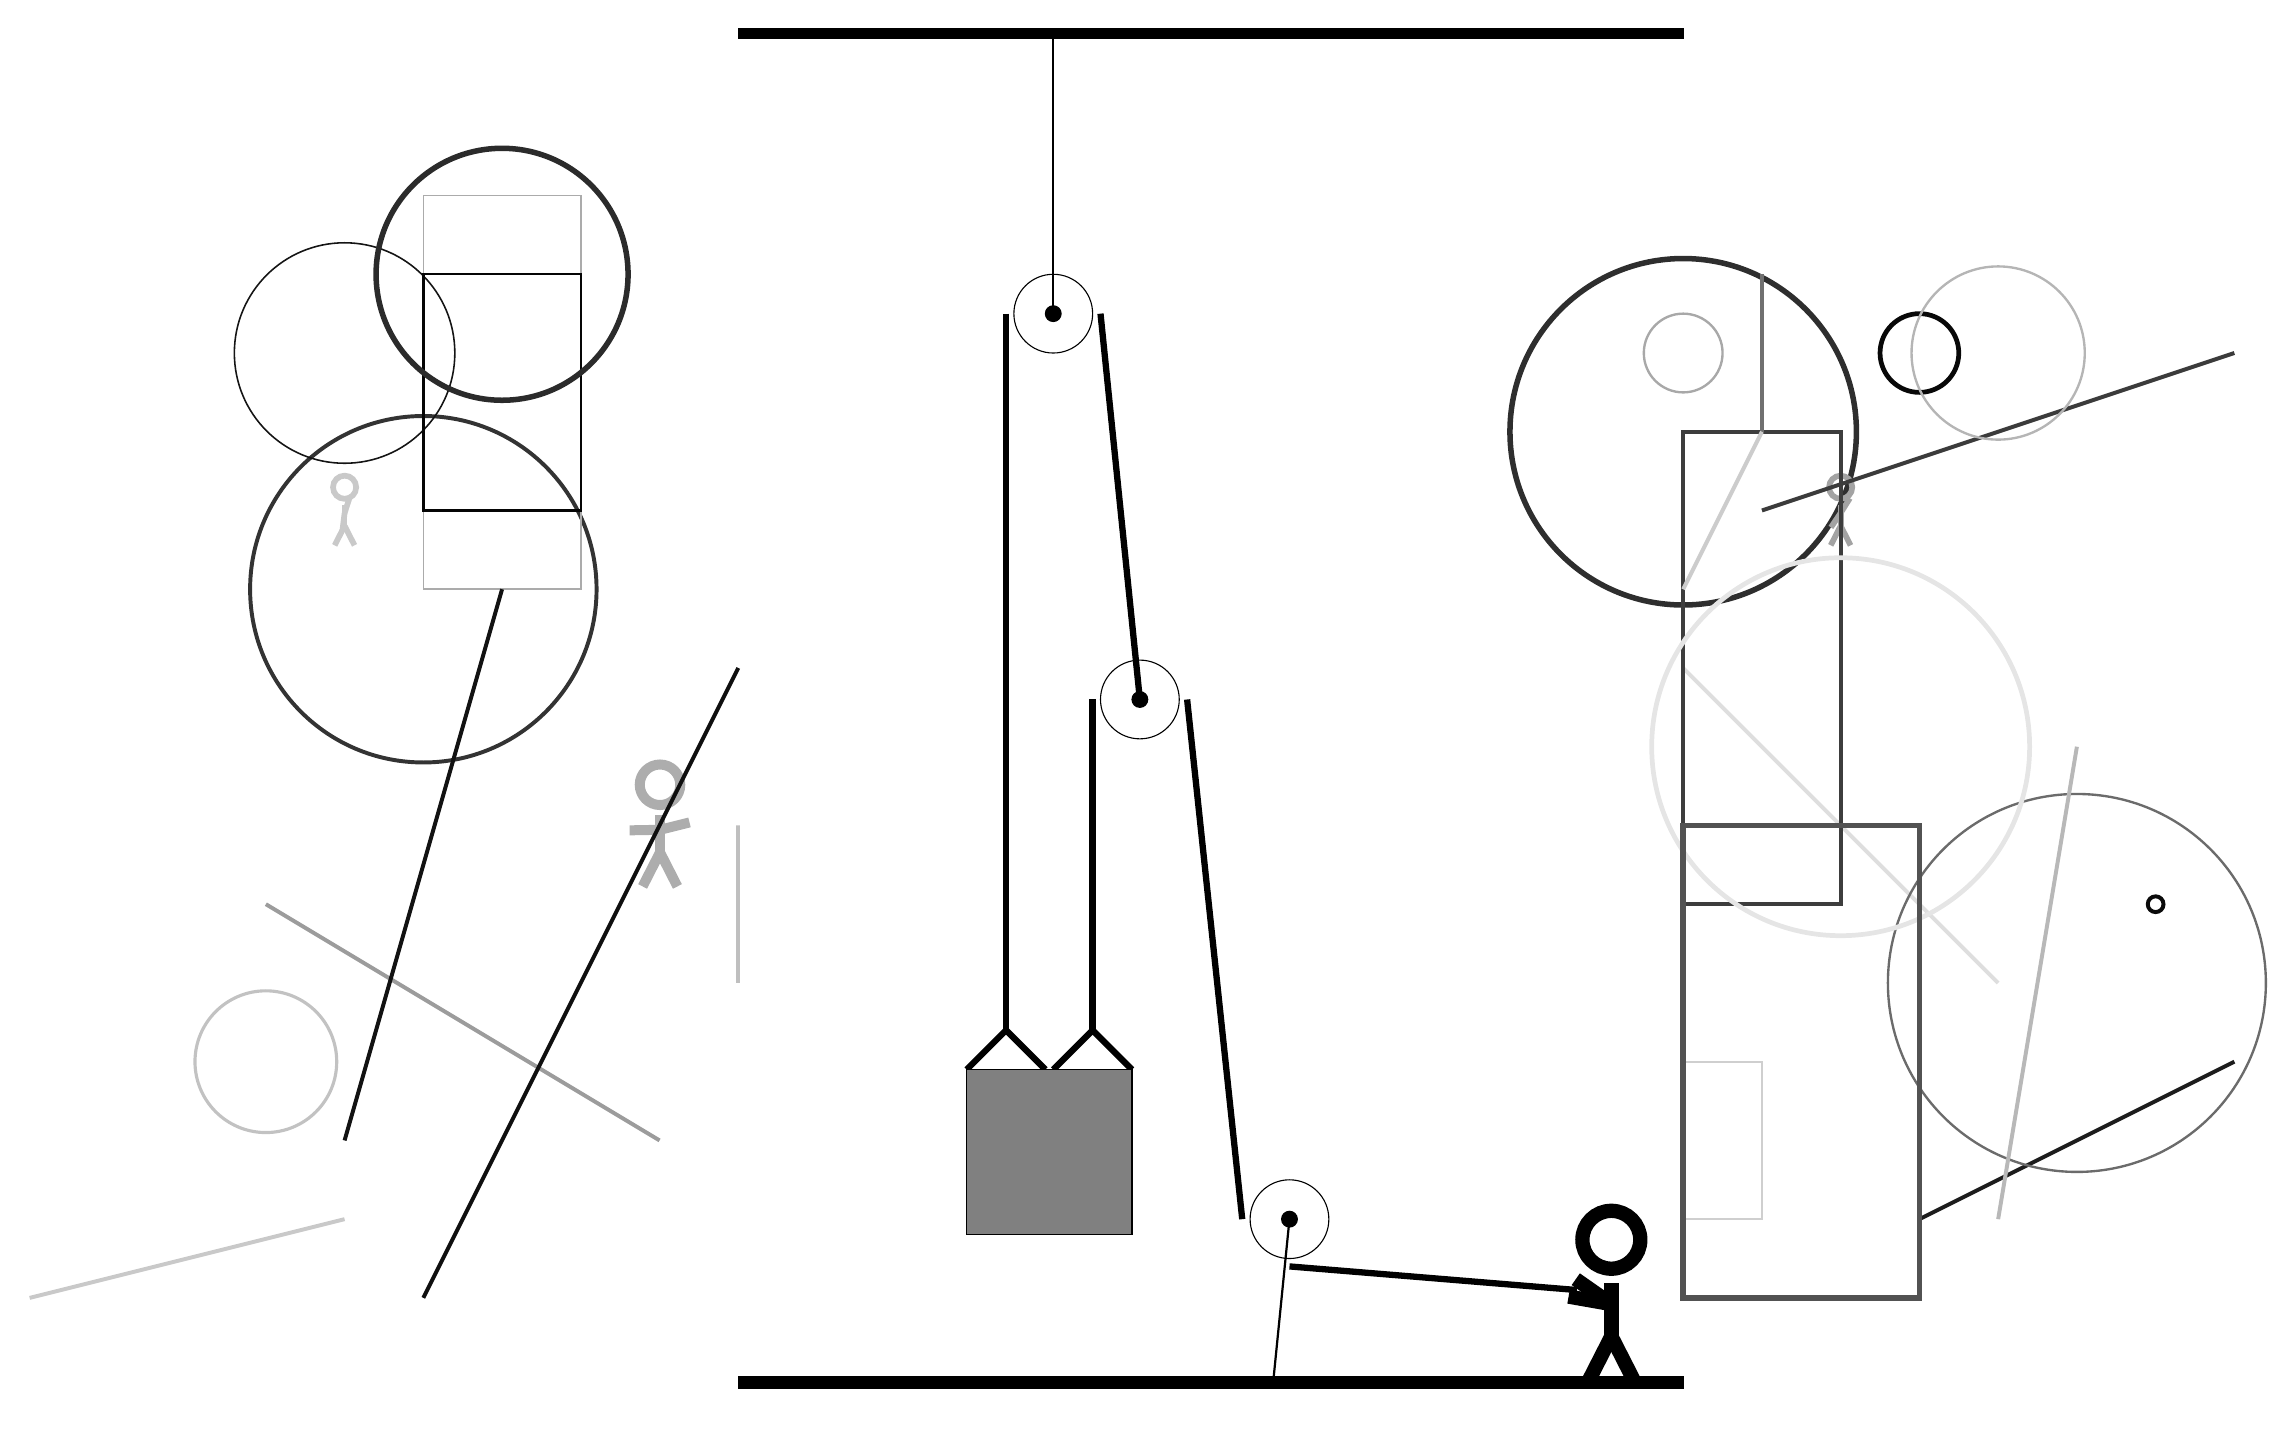
\begin{tikzpicture}
			%%%%% START %%%%%
			
			\draw[fill=black] (-2, 14) rectangle (10, 14.125);
			
			\draw (2, 10.5) circle (0.5);
			\draw[fill=black] (2, 10.5) circle (0.1);
			\draw[thick] (2, 10.5) -- (2, 14);
			
			\draw (3.1, 5.6) circle (0.5);
			\draw[fill=black] (3.1, 5.6) circle (0.1);
			
			\draw (5, -1) circle (0.5);
			\draw[fill=black] (5, -1) circle (0.1);
			\draw[thick] (5, -1) -- (4.8, -3);
			
			\draw[line width = 0.8mm]  (0.9, 0.9) -- (1.4, 1.4) -- (1.9, 0.9);
			\draw[line width = 0.8mm]  (2.0, 0.9) -- (2.5, 1.4) -- (3.0, 0.9);
			\draw[fill=black!50] (0.9, 0.9) rectangle (3.0, -1.2);
			
			\draw [line width=0.5mm, color=black!80](-6, 7) circle (2.2);
			
			\draw[line width=0.5mm, color=black!13](14, 2) -- (10, 6);
			\draw[line width=0.2mm, color=black!33] (-4, 7) rectangle (-6, 12);
			\draw [line width=0.6mm, color=black!97](13, 10) circle (0.5);
			\draw [line width=0.7mm, color=black!82](10, 9) circle (2.2);
			\draw[line width=0.5mm, color=black!25] (-2, 2) rectangle (-2, 4);
			
			\node[line width=0.2mm, color=black!32] at (-3, 4) {\Strichmaxerl[7][1][14]};
			\node[line width=0.3mm, color=black!36] at (12, 8) {\Strichmaxerl[4][56][58]};
			\draw[line width=0.5mm, color=black!89](13, -1) -- (17, 1);
			\draw [line width=0.5mm, color=black!96](16, 3) circle (0.1);
			\draw [line width=0.3mm, color=black!58](15, 2) circle (2.4);
			
			\draw[line width=0.5mm, color=black!76] (12, 9) rectangle (10, 3);
			\draw[line width=0.5mm, color=black!56](11, 11) -- (11, 9);
			
			\draw [line width=0.2mm, color=black!92](-7, 10) circle (1.4);
			\draw[line width=0.5mm, color=black!77](11, 8) -- (17, 10);
			\draw [line width=0.3mm, color=black!29](14, 10) circle (1.1);
			
			\node[line width=0.5mm, color=black!21] at (-7, 8) {\Strichmaxerl[4][83][72]};
			\draw [line width=0.3mm, color=black!34](10, 10) circle (0.5);
			\draw[line width=0.5mm, color=black!20](11, 9) -- (10, 7);
			\draw[line width=0.5mm, color=black!39](-3, 0) -- (-8, 3);
			\draw[line width=0.5mm, color=black!28](15, 5) -- (14, -1);
			\draw[line width=0.5mm, color=black!94](-2, 6) -- (-6, -2);
			\draw [line width=0.6mm, color=black!10](12, 5) circle (2.4);
			\draw[line width=0.3mm, color=black!98] (-4, 8) rectangle (-6, 11);
			\draw [line width=0.7mm, color=black!83](-5, 11) circle (1.6);
			
			\draw[line width=0.3mm, color=black!19] (10, -1) rectangle (11, 1);
			\draw[line width=0.7mm, color=black!68] (10, -2) rectangle (13, 4);
			\draw [line width=0.4mm, color=black!24](-8, 1) circle (0.9);
			\draw[line width=0.5mm, color=black!21](-7, -1) -- (-11, -2);
			\draw[line width=0.5mm, color=black!93](-5, 7) -- (-7, 0);
			
			\draw[line width = 0.8mm] (1.4, 10.5) -- (1.4, 1.4);
			\centerarc[line width = 0.8mm](2, 10.5)(0:180:0.6);
			\draw[line width = 0.8mm] (2.6, 10.5) -- (3.1, 5.6);
			\draw[line width = 0.8mm] (2.5, 5.6) -- (2.5, 1.4);
			\centerarc[line width = 0.8mm](3.1, 5.6)(0:180:0.6);
			\draw[line width = 0.8mm] (3.7, 5.6) -- (4.4, -1);
			\centerarc[line width = 0.8mm](5, -1)(180:270:0.6);
			\draw[line width = 0.8mm] (5, -1.6) -- (8.65, -1.9);
			
			\node at (9, -2) {\Strichmaxerl[10][-35][170]};
			
			\draw[fill=black] (-2, -3) rectangle (10, -3.15);
			
			%%%%% END %%%%%
		\end{tikzpicture}
	\end{figure}	
\end{document}